%-----------------------------------------------------------------------------
%
%               Template for sigplanconf LaTeX Class
%
% Name:         sigplanconf-template.tex
%
% Purpose:      A template for sigplanconf.cls, which is a LaTeX 2e class
%               file for SIGPLAN conference proceedings.
%
% Guide:        Refer to "Author's Guide to the ACM SIGPLAN Class,"
%               sigplanconf-guide.pdf
%
% Author:       Paul C. Anagnostopoulos
%               Windfall Software
%               978 371-2316
%               paul@windfall.com
%
% Created:      15 February 2005
%
%-----------------------------------------------------------------------------


\documentclass[10pt,nocopyrightspace]{sigplanconf}

% The following \documentclass options may be useful:
%
% 10pt          To set in 10-point type instead of 9-point.
% 11pt          To set in 11-point type instead of 9-point.
% authoryear    To obtain author/year citation style instead of numeric.

\usepackage[normalem]{ulem}
\newcommand{\Comment}[1]{\textcolor{red}{\bf #1}}
%\renewcommand{\iff}{\ensuremath{\mathrm{iff}}}
\usepackage{tabularx}
\usepackage{fancyhdr}
\usepackage{float}
\usepackage{graphicx}
\usepackage{epstopdf}
\usepackage[labelfont=bf]{caption}
\usepackage{subcaption}
\usepackage{natbib}
\usepackage{balance}

\epstopdfsetup{update}

\begin{document}

%\titlebanner{}        % These are ignored unless
\preprintfooter{}   % 'preprint' option specified.

\title{Automatic Multi-Threading Through HDL Transformation}
\subtitle{}

\authorinfo{Wenyu Tang}
           {University of California, Berkeley}
           {wenyu@eecs.berkeley.edu}

\maketitle

\begin{abstract}
Digital hardware frontend specification is defined by two extremes - RTL specification and HLS specification. RTL specifcation produces highly optimized designs, but requires extremely verbose low level specification on the part of the designer. On the otherhand, HLS specification requires much less verbose high level specification from the designer, but does not produce well optimized designs. In this thesis, I present a middle ground that captures the pros of these two extremes - a system in which the designer specifies a basic datapath and uses a tool to automatically apply optimizations to that basic datapath.
\end{abstract}

\section{Introduction}
Over the past 30 years, progress in programming languages has greatly increased the productivity of software design by moving low level resource allocation and optimization tasks away from the programmer to the compiler or interpreter.  In contrast, increase in productivity of digital hardware logic design has largely stalled after the transition from schematic based specification to to Register Transfer Level (RTL) specification languages such as Verilog or VHDL for front end specification.

While RTL specification succeeds in providing the digital logic designer with a specification that is higher level than transistor level or gate level schematic specification, RTL specification is still quite a low abstraction level and requires the designer to provide a very detailed specification of the design. High Level Synthesis (HLS) has been an attempt to increase the productivity of digital logic designers by going to a much higher level of specification than RTL and automatically synthesizing all of the details of the design. However, the higher abstraction level of HLS comes at the cost of unsatisfactory performance, area, and power characteristics due to inefficiencies introduced in the automatic logic synthesis process.

In this thesis, I propose a system in which the designer specifies a basic functional datapath in a RTL like manner and selects optimizations that should be applied to the design, which will then be automatically applied through a tool. This middle ground method increases digital logic designer productivity without producing designs with unacceptable performance, power, and area characteristics like HLS. I implement two examples of such a system, AutoMArch and AutoFAME, and I describe their implementation and example applications.


\section{Related Work}

\begin{figure*}
	\centering
    \resizebox{1.5\columnwidth}{!}{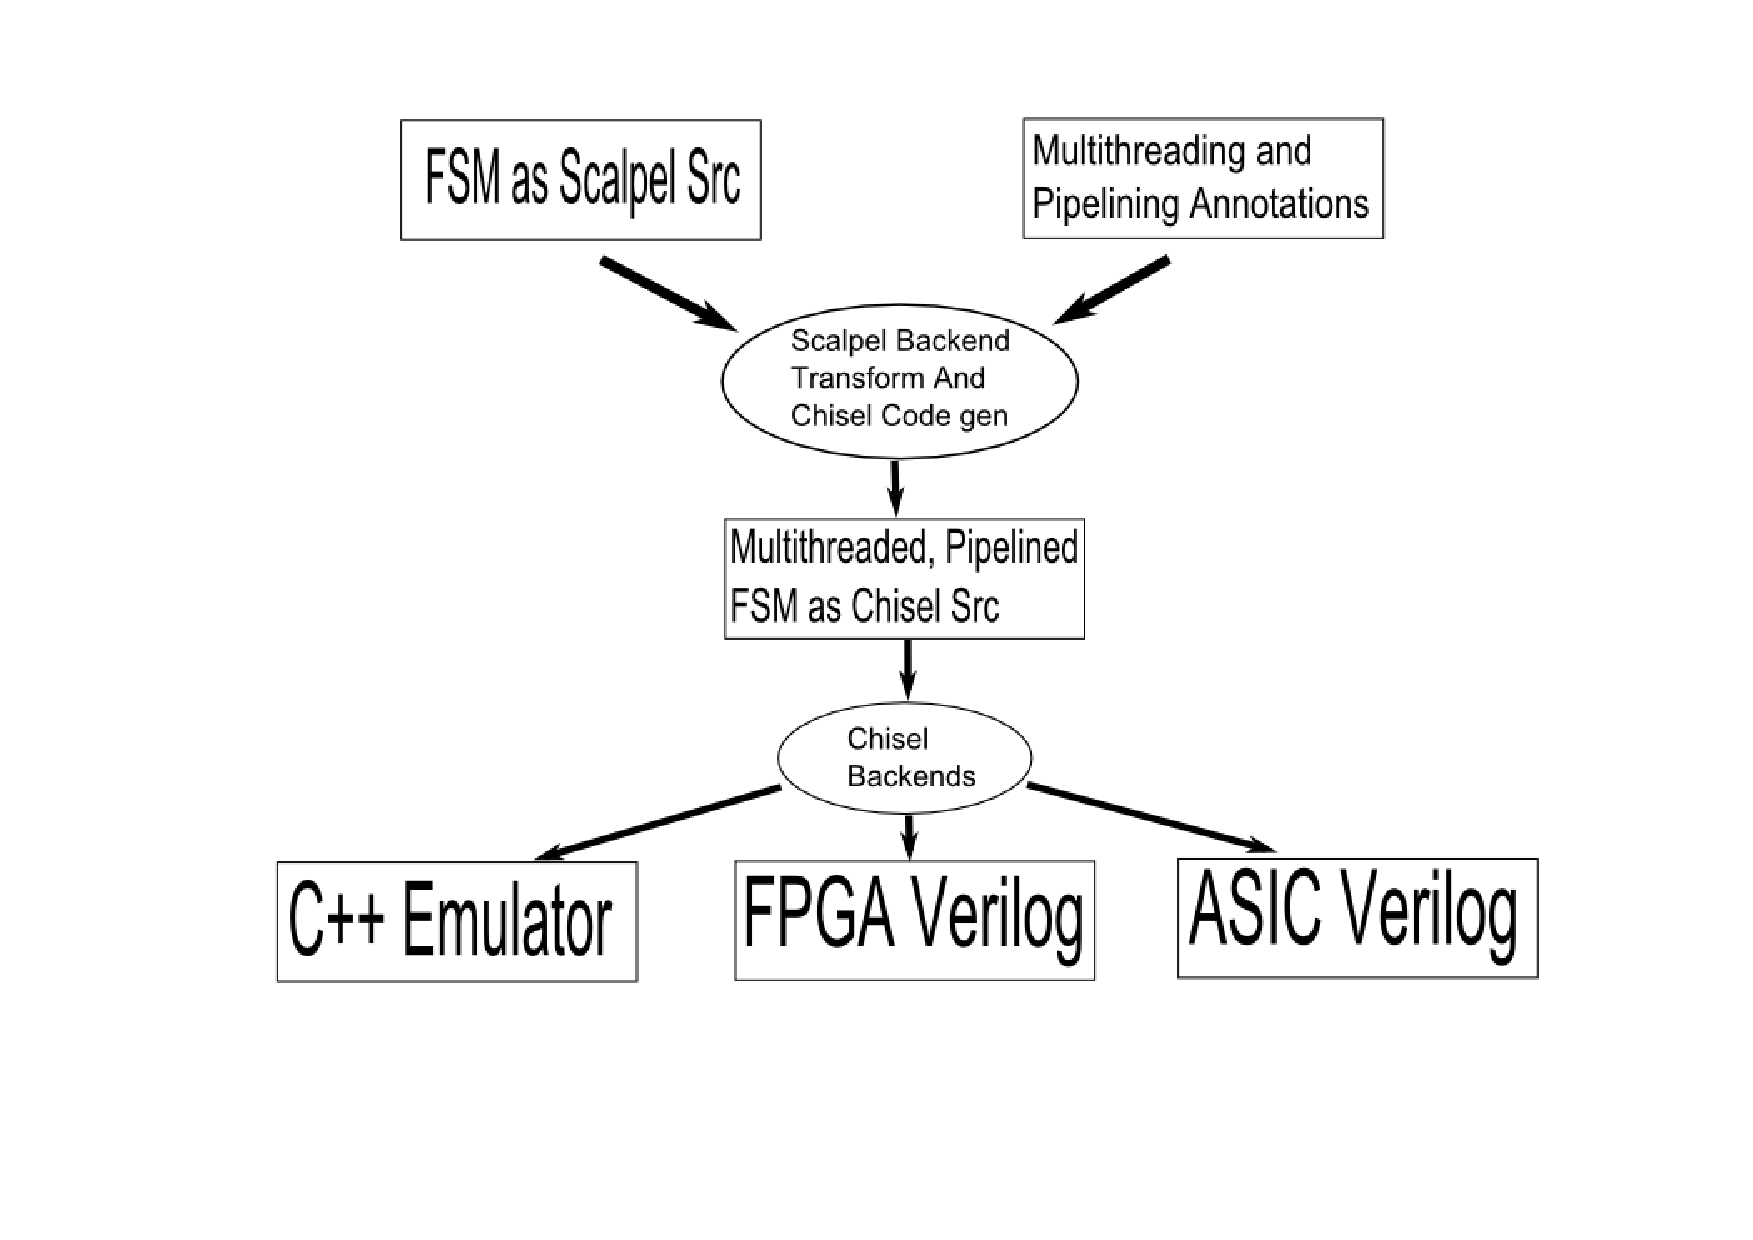
\includegraphics{figures/workflow}}
    \caption{Overall Tool Flow}
	\label{fig:workflow}
\end{figure*}

\section{Proposed Solution}
HLS produces designs with unacceptable performance, power, and area characteristics because the synthesis tool has to solve the computationally difficult problem of formulating a datapath that executes the dataflow graph and fits within the given performance, power, and area constraints. HLS tools do synthesize well optimized designs for specific patterns that occur in the high-level specification, so hardware designers working with HLS find themselves tuning high-level code to make specific synthesis tools produce exactly the datapath they want. 

This is clearly a case of automation trying to do too much. The HLS tools have a hard time formulating optimized datapaths, so the designers have to essentially tell the HLS tools what datapath they should use in a roundabout way by tuning the high-level specification. Clearly, designers would be more productive if they can specify the datapath directly. 

It seems like this conclusion tells us that designers should just do logic design using RTL in the traditional manner. However, much of traditional RTL specification deals with issues outside of simple datapath design. Logic designers spend much of their time specifying additional logic required to make the datapath fit performance, power, and area constraints. Some common optimization techniques include time-multiplexing functional units, pipelining, multi-threading, out-of-order execution, etc. These commonly used datapath optimization techniques can be captured as algorithms and applied automatically.

This thesis proposes a system in which the designer creates a RTL specification of the base functional datapath and separately specifies a series of optimizations to be performed on the datapath. Then automatic tools that know how to generically apply common optimization techniques can apply the specified optimizations to the base datapath and produce an optimized gate level specification to be fed into the next step in the IC design flow which may be physical design, fpga synthesis, or simulation. This system of specification will hence be referred to as Automatic Functional Datapath Optimization (AFDO). AFDO allows the designer to specify designers to specify a digital circuit with higher productivity than RTL specification without incurring the performance, power, and area penalties of HLS specification.

The automatic optimization tools discussed above work in the following manner. First, some initial processing transforms the RTL specification of the base datapath into a node graph data structure, where each node represents a digital circuit component(wire, combinational logic block, or state element) and each node contains input and consumer pointers to other nodes representing the topology of the circuit. Second, the tools implement the specified optimizations by modifying this node graph - creating new nodes, changing input/consumer pointers, copying existing nodes, etc. Third, the tool outputs the modified circuit in some specified representation

Although AFDO can be implemented if the base datapath is specified in discrete event simulation based RTL languages such as Verilog or VHDL, it is better for the base datapath should specified in a structural construction based RTL language such as Chisel. First, as mentioned in \ref{section:RTLCons}, discrete event simulator semantics are not particularly well suited for digital hardware specification and create a host of problems for the designer. Second, creating a node graph representation of the base datapath is much easier in structural construction based HDL languages such a Chisel as there is a one to one mapping between language construct and nodes in the node graph. In the case of Chisel, the automatic tools can directly operate on Chisel’s internal node graph data structure. In discrete event simulation based RTL languages, we have to first send the RTL specification through a gate level synthesis tool before we can construct the node graph data structure. This makes preserving names difficult and prevents the designer from using RTL level simulations of the automatically optimized designs. All of the automatic optimization tools discussed in the following sections apply transformations to base datapaths specified in Chisel or a reduced Chisel like RTL specifically designed to demonstrate AFDO.

AFDO increases logic designer productivity by addressing both limitations of RTL specification covered in \ref{section:RTLCons}. By usings a structural construction based RTL language like Chisel to specify the base functional datapath, the problems caused by discrete event simulator semantics are eliminated. By allowing the designer to specify only the base functional datapath, which is generally much less complex than the optimized design, and applying optimizations automatically, source code verbosity and algorithm obfuscation is eliminated. Now the designer can specify designs much faster and with fewer errors as he only has to specify the simple base functional datapata and use automatic tools to systematically apply the desired optimizations. Additionally, AFDO allows designers to more easily do design space exploration as they can produce new design points by simply selecting different optimization options for the automatic tools to apply instead of rewriting obfuscated RTL for each new design point. For example, adding a pipeline stage to a processor design in RTL is generally non-trivial in RTL because the pipeline control logic is entwined within the datapath specification. If the designer specifies a base functional 1 stage version of the processor and uses an automatic tool to pipeline the processor, adding a pipeline stage would be trivial on the part of the designer as he would simply have to tell the automatic pipeline tool to generate one more stage.

At the same time, AFDO retains performance, power, and area benefits of RTL specification by preserving a high level of correlation between language constructs and the generated hardware. The generated datapath is simply the base functional datapath modified with the designer specified optimizations. Unlike HLS, the designer knows the number and types of functional units used in the datapath as well as the state elements that are present in the datapath along with how those state elements are updated.

\section{Technical Approach}
\subsection{Input FSM Specification}
The input minimal FSM can be an arbitrary FSM with the following restrictions:

{\bf (1)} The input FSM must communicate to the outside world through ready/valid ports  

{\bf (2)} The designer cannot use input valid or output ready signals as inputs to any part of their circuit

{\bf (3)} Any functional units that may take more than one clock cycle to return responses(caches, multipliers, dividers, etc) must be accessed through the Variable Latency Unit Interface discussed below.

\subsubsection{IO Semantics}
When input ready or output valid is driven high by the input FSM, this implicity signals to the tool that the input FSM requires the use of the input or output port on the current state update. Thus, the tool generates logic that examines the input ready or output valid and stalls the pipeline if the corresponding input valid or output ready is not driven high by external modules. The designer should design the input FSM so that input readies and output valids are only driven high when absolutely necessary to avoid unnecessary stalling the automatically multi-threaded and pipelined version of the circuit.

\begin{figure}
	\centering
    \resizebox{\columnwidth}{!}{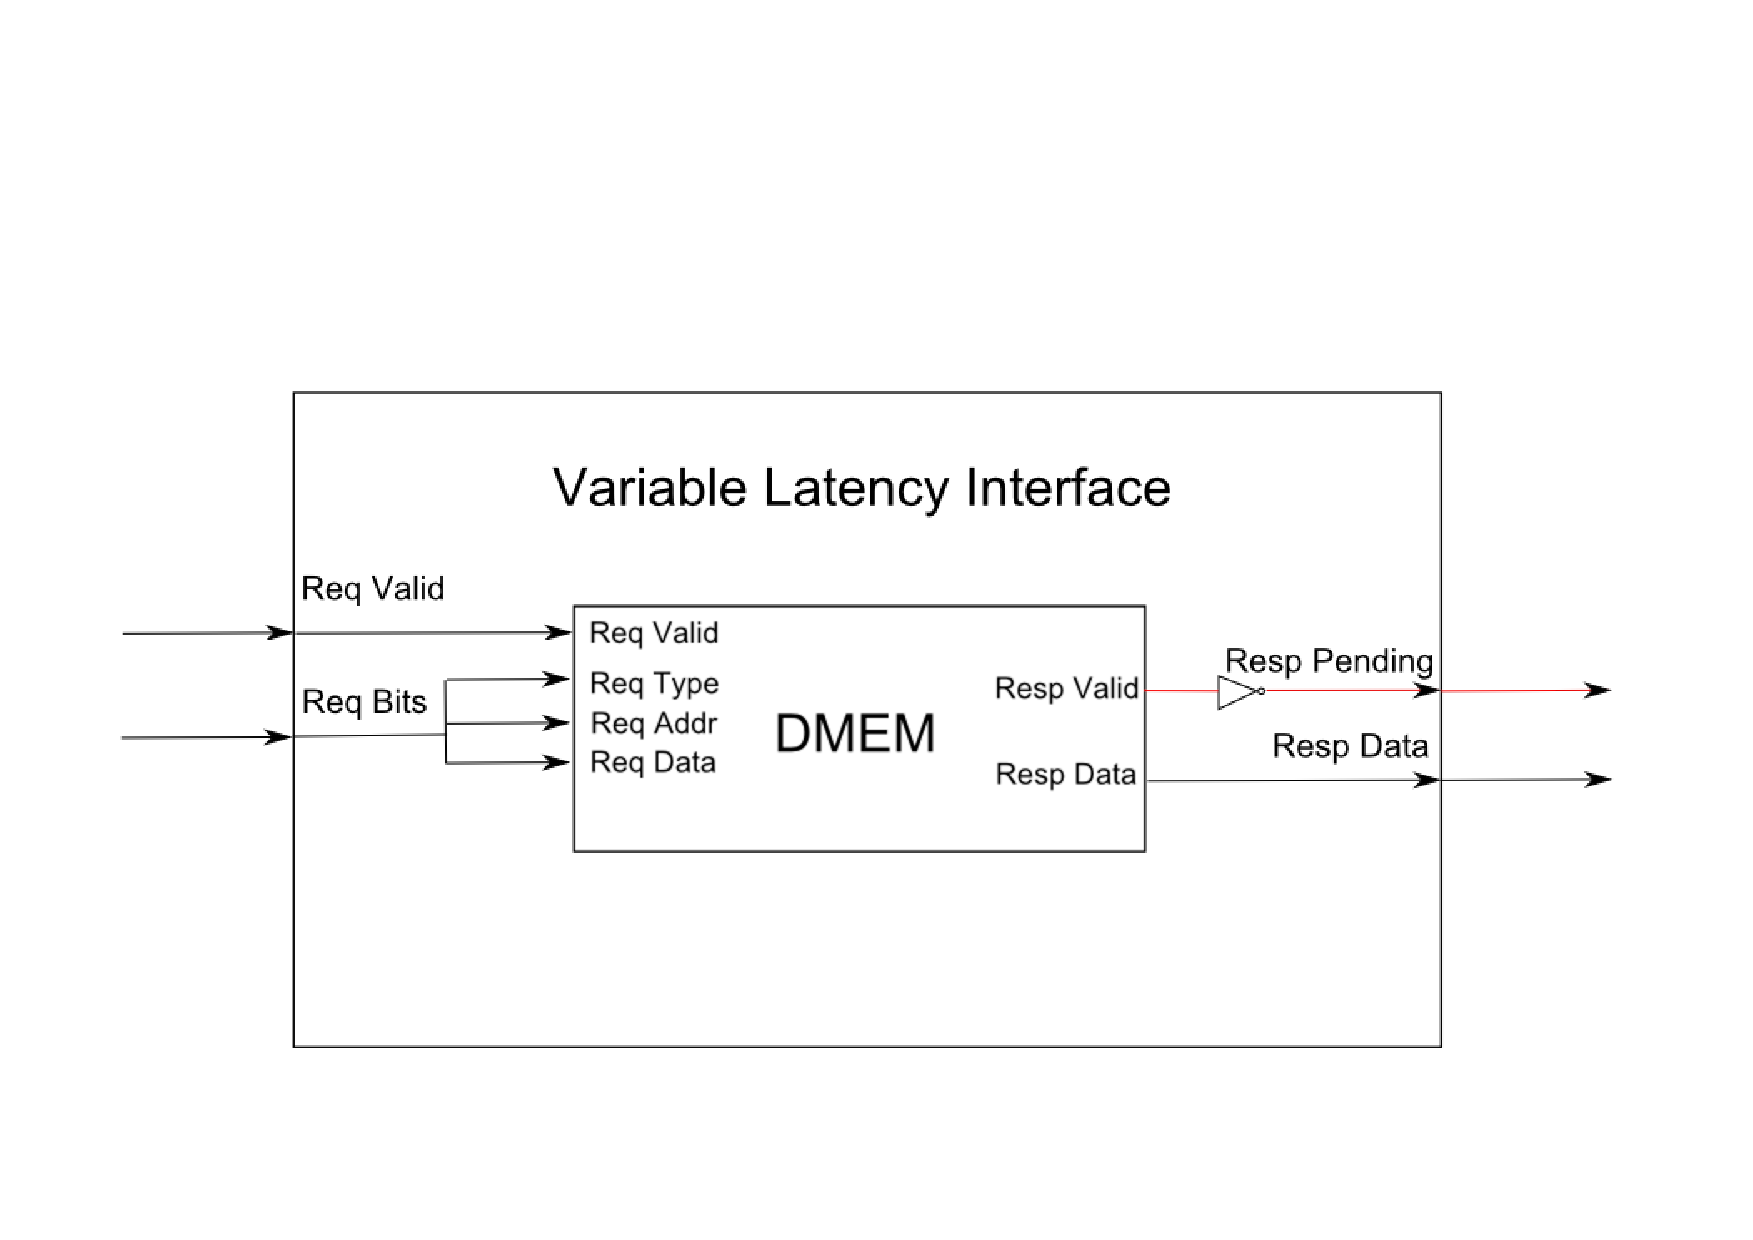
\includegraphics{figures/TransactionalInterface}}
    \caption{{\bf Single Thread View of Variable Latency Unit Interface} Black wire are user facing IO, red wires are tool facing IO}
	\label{fig:VarLatIO}
\end{figure}

\subsubsection{Variable Latency Unit Interface}
In order to accomodate caches and long latency arithmetic units in the minimal FSM specification that is not allowed to have any optimization or control logic implemented, the tool provides the Variable Latency Unit Interface. The designer should access any caches or long latency arithmetic units through a Variable Latency Unit Interface and treat that Variable Latency Unit Interface like a piece of combinational logic in the input FSM specification. IE the designer should not use the Resp Pending port of the Variable Latency Unit Interface to drive any part of their circuit and should pretend that the Variable Latency Unit Interface always gives a valid response immediately. The tool will automatically generate control logic that deals with the Variable Latency Unit Interface not immediately outputting a valid response.

When the tool does the multithreading transformation, each Variable Latency Unit Interface in the input minimal FSM is replicated n times, where n is the number of threads. It is up to the designer to create glue logic that deals the copies of the Variable Latency Unit Interfaces in a top level module that instantiates the automatically multi-threaded module. The designer can instantiate n copies of the functional unit, one for each Variable Latency Unit Interface, or can create additional logic that multiplexes all copies of the Variable Latency Unit Interface onto a single functional unit.

\subsection{Minimal FSM Transformation}
Given an input minimal FSM, the tool analyzes the node graph that represents the FSM and modifies the node graph to generate a multi-threaded, pipelined design that is functionally equivalent to n copies of the input FSM, where n is the number of threads.

In order to make analysis of the input FSM easier, the tool breaks up the state elements into read and write ports. This results in an acyclic node graph in which data flows from the state element read ports and the input data ports to the state element write ports and output data   ports. For the figures in this section, state elements are draw as separate "r" and "w" pieces.

Figure \ref{fig:initialFSM}. and Figure \ref{fig:finalFSM}. show an example initial input minimal FSM and the final multi-threaded, pipelined FSM after the transformation. The rest of this section describes the transformations that are performed.

\begin{figure}
	\centering
    \resizebox{\columnwidth}{!}{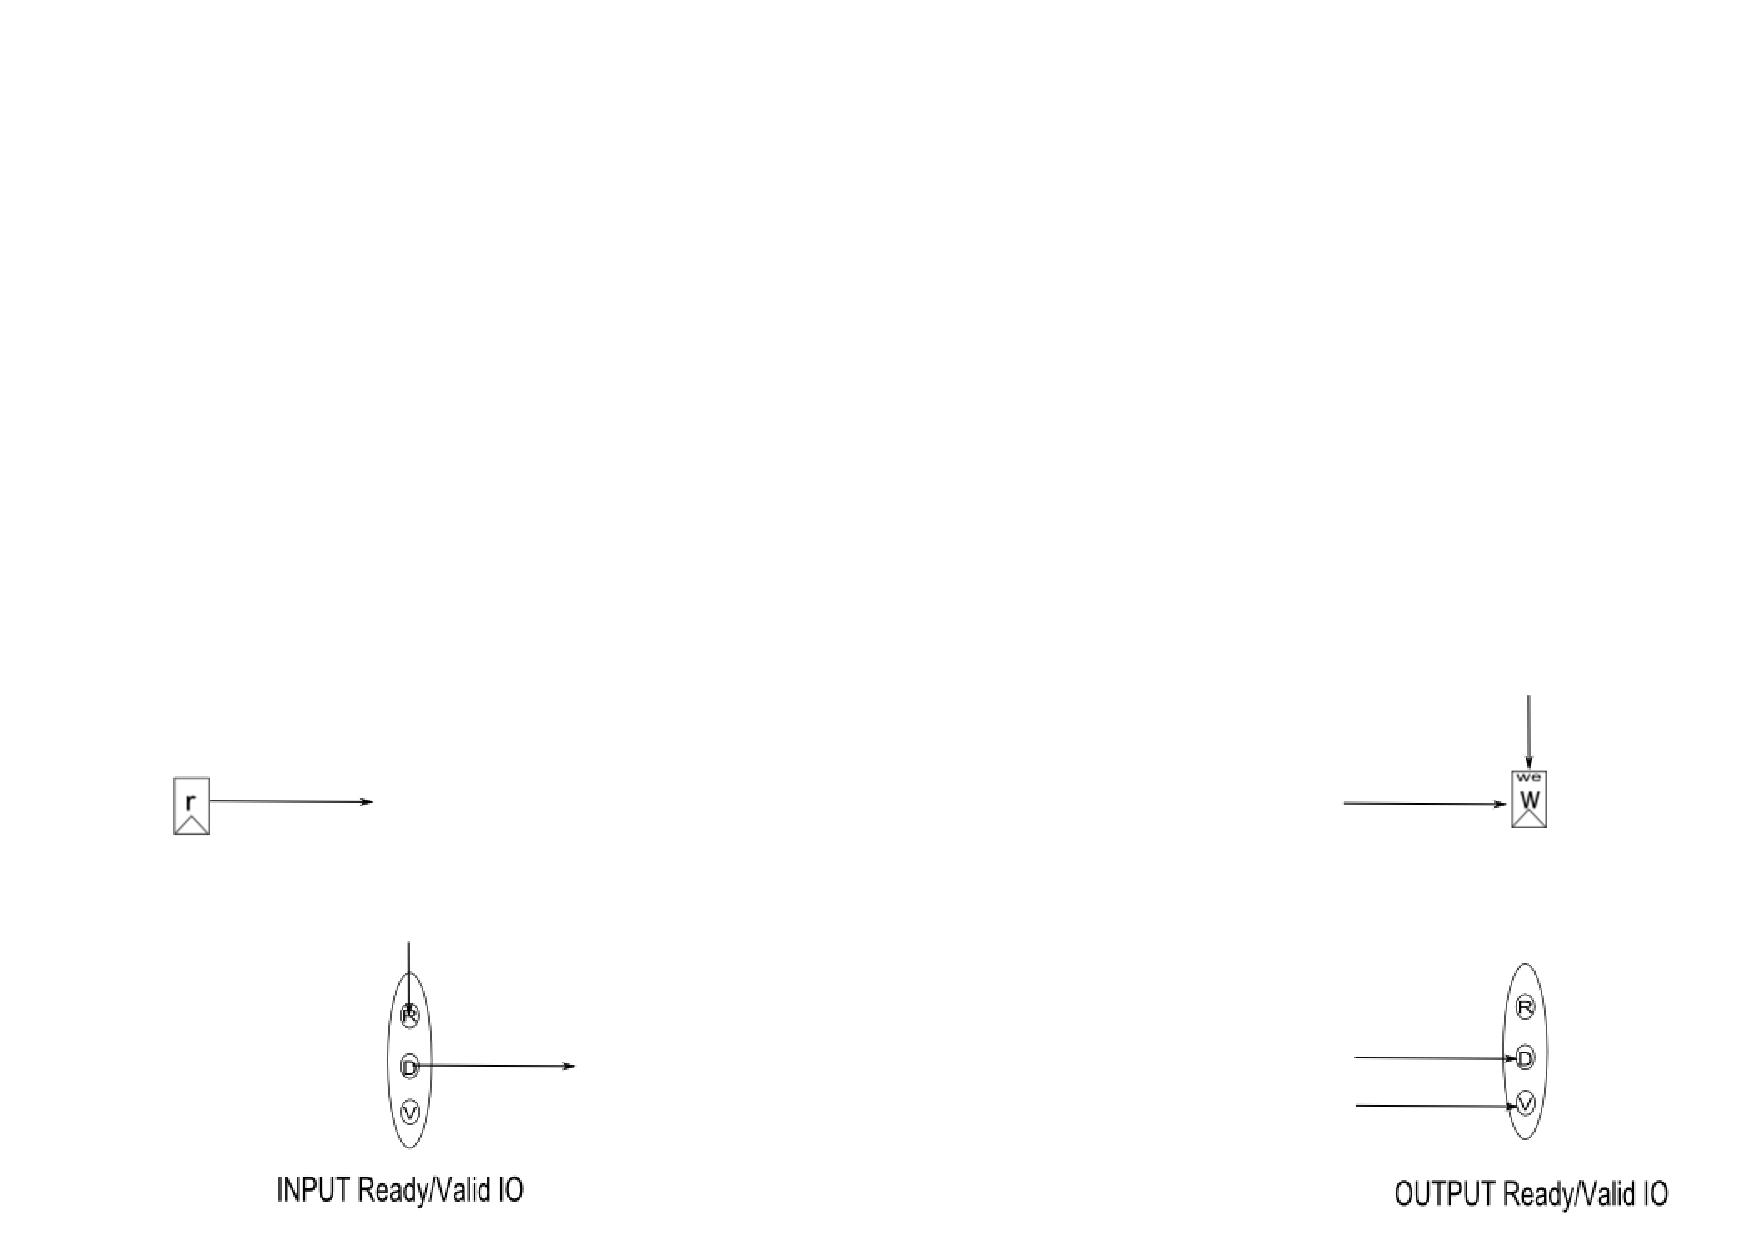
\includegraphics{figures/initialFSM}}
    \caption{{\bf Input Minimal FSM} The input FSM consists of one register, one input port, and one output port. The register is split up into read and write ports. The combinational logic is not shown.}
	\label{fig:initialFSM}
\end{figure}

\begin{figure}
	\centering
    \resizebox{\columnwidth}{!}{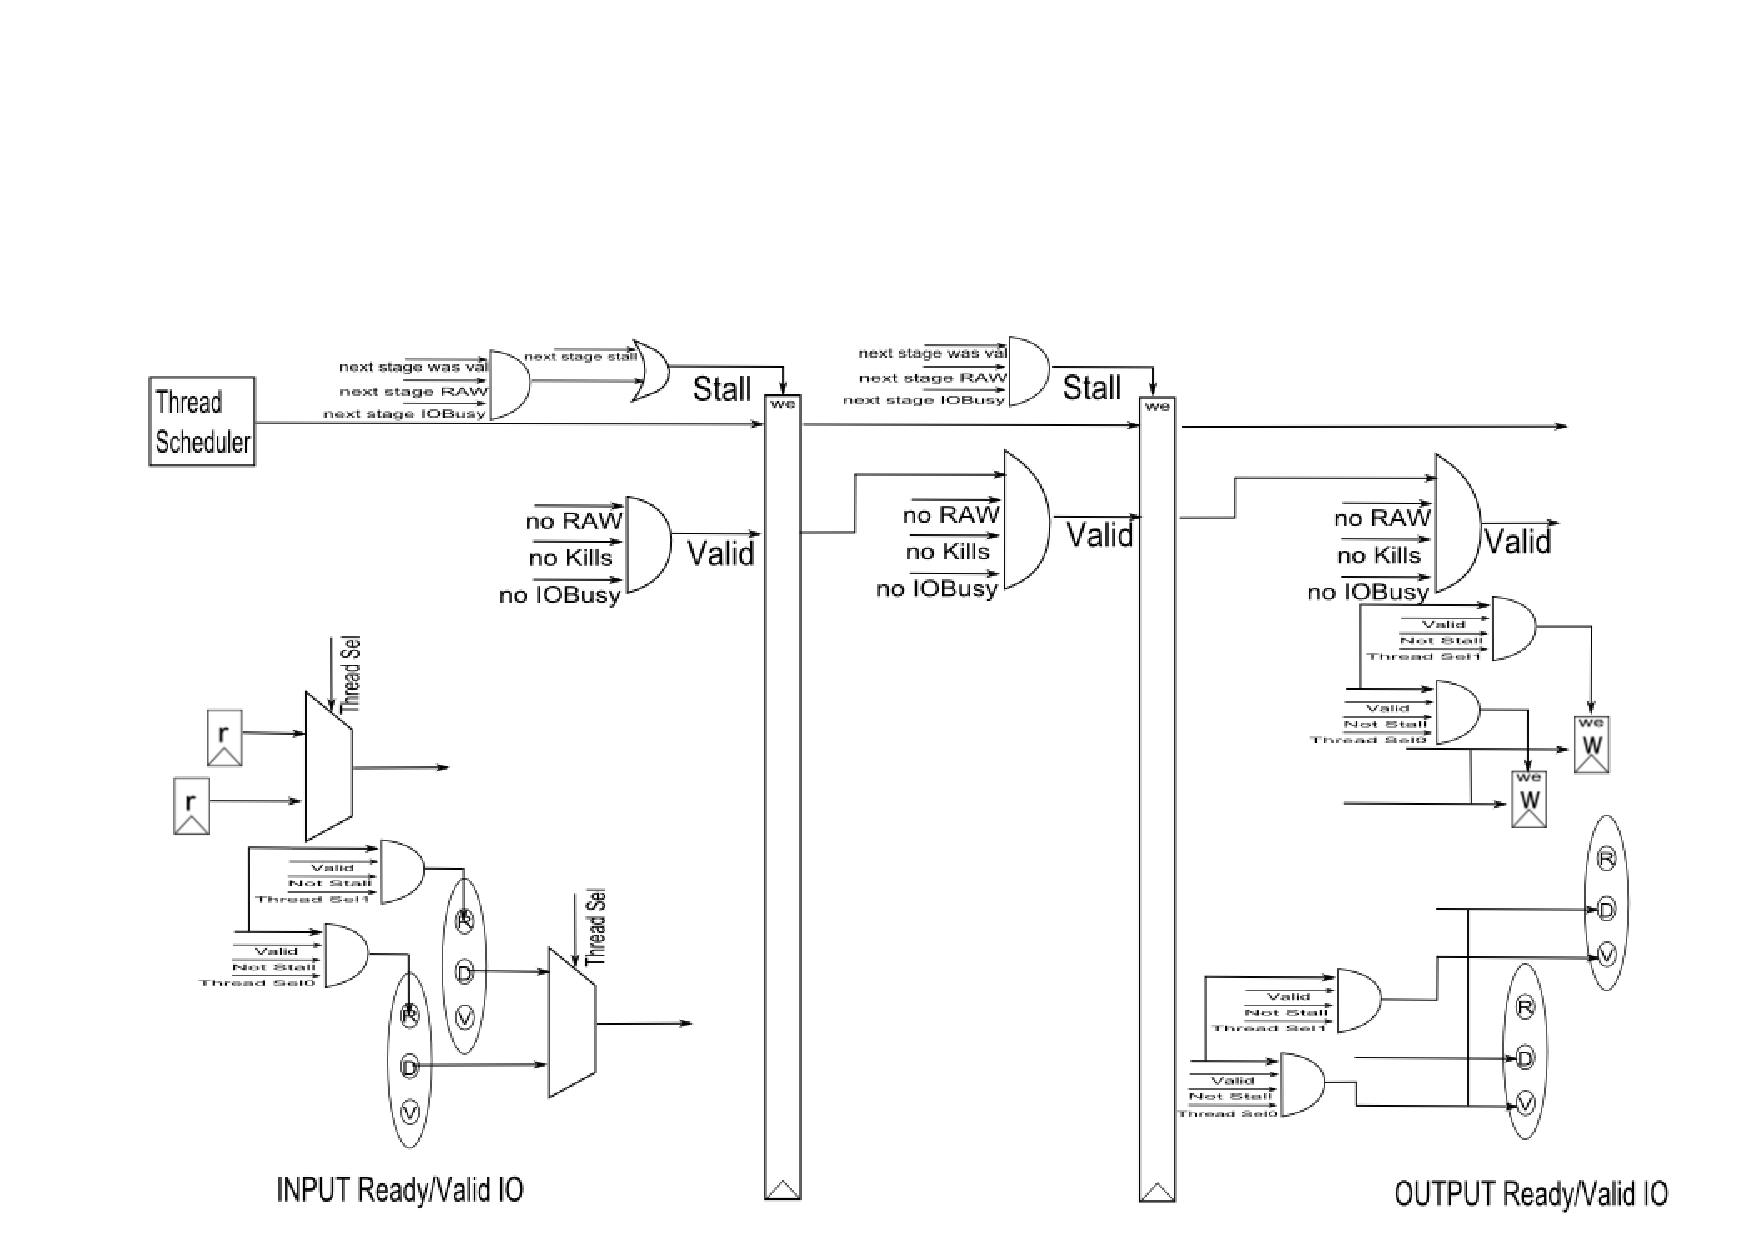
\includegraphics{figures/finalFSM}}
    \caption{{\bf Final Multi-threaded, Pipelined FSM} This is a 2 thread, 3 stage version of the input FSM with all of the generated control logic shown. The cominational logic is not shown.}
	\label{fig:finalFSM}
\end{figure}

\subsection{State and IO replication}
\label{sec:replication}
Given a user specification of n threads, the tool first replicates the IO ports the state elements n times. The input ready signals, output data signals, and the output valid signals of the replicated IO elements are driven by the corresponding original IO port signals. The state element write data signals, and state element write enable signals of the replicated state elements are drive by the corresponding original state element write signals. 

A mux is placed infront of the input data signals and all consumers of the original input data signal is now driven by this mux. Similarly, a mux is placed infront of the replicated state element read data signals and all consumers of the original read data signal is now drive by this mux.

\subsection{Pipeline Register Insertion}
Given a user specification of m pipeline stages, the tool inserts m - 1 pipeline registers into the design. The tool automatically finds a legal placement of the registers that satisfy the following rules:

{\bf (1)} Every combinational logic node has all input signal with the same stage number.  

{\bf (2)} The stage number of every combinational logic node's output signal is equal to the shared stage number of its input signals.

{\bf (3)} There are two ways to determine the stage number of a node. One way is to trace through the node's inputs to a pipeline register and set the stage number of the node equal to the stage number of that pipeline register. Another way is to trace through the node’s consumers to a pipeline register and set the stage number of the node equal to the stage number of that pipeline register {\tt -}  1. For all nodes in the graph, the stage number of the node obtained through both methods must be the same.

Then the tool automatically optimizes the pipeline register placement with regards to critical path delay by balancing the longest path delays for each pipeline stage. The details of how this is done will not be discussed in the paper as it was part of the previous automatic pipelining project.

\subsection{Control Logic Generation}
The tool then inserts logic that generates thread select and pipeline control signals. 

\subsubsection{IOBusy Signals}
An IO port is considered busy if it belongs to the thread that matches the thread ID signal in the IO port's stage and if the input ready/output valid signal is driven high, which implicitly signals that the data from this port is needed to be consumed/produced, and the input valid/output ready signal is driven low by an outside module, which indicates that the port is not available.

\subsubsection{RAW Hazard Signals}
A read port belonging to thread N, stage X is considered to have a RAW hazard if a pipeline stage Y is valid, has the same thread ID as stage X, and contains a transaction that could write to any write port that belongs to the same state element as the read port.

\subsubsection{Kill Signals}
A stage is killed if a Variable Latency Unit IO in that stage drives RespPending high and the thread ID signal of the stage equals the thread that Variable Latency Unit IO belongs in.

\subsubsection{ThreadID signals}
The tool pipelines the thread ID signal generated by the thread scheduler so that it is available for each pipeline stage. The thread ID signal in each pipeline stage is wired into the muxes generated in \ref{sec:replication}. The input ready signals, output valid signals, Variable Latency Unit Interface Req Valid signals, and state element write enable signal are masked with the thread ID signal for the pipeline stage they belong in.

\subsubsection{Valid Signals}
The tool generates a valid signal for each pipeline stage. Each pipeline stage is currently valid if the previous pipline stage was valid on the last clock cycle, no state element read ports in this pipeline stage has a RAW hazard, no IO port in this stage is busy, and there are no kill signals triggered in this stage. The input ready signals, output valid signals, Variable Latency Unit Interface Req Valid signals, and state element write enable signal are masked with the valid signal for the pipeline stage they belong in.

\subsubsection{Stall Signals}
The tool generates a stall signal for each pipeline stage. When a pipeline stage is stalled, the contents of that pipeline stage does not progress into the next pipeline stage. The boolean equation for stage X's stall signal = stage X + 1 is stalled OR (stage X was valid last cycle AND (a read port in stage X+1 has a RAW hazard OR a IO port in stage X+1 is busy)). The input ready signals, output valid signals, Variable Latency Unit Interface Req Valid signals, and state element write enable signal are masked with the valid signal for the pipeline stage they belong in. 

\section{Results}
For evaluation of the tool, I created simple RISC processor in Scalpel and explored the design space of number of threads (1 - 4), number of pipeline stages (1 - 4), and fixed vs dynamic interleave. The base RISC processor is a classic RISC machine that contains a ICache with a miss latency of 4 cycles, which is accessed through a Variable Latency Interface, and a magic single cycle DMem. 

In order to evaluate how effective the generated multi-threaded designs are at hiding the latencies of long latency functional units in general, which is one of the primary advantages of multi-threading, the ICache is made to pseudo randomly miss based on the output of a LFSR. Each thread accesses its own private ICache through the Variable Latency Unit Interface. This gives a representative evaluation of multi-threaded design effectiveness regardless of the quality of the benchmark program used on the RISC processor.

The metric for performance used is Throughput/Area, which can be broken down into $Task/Cycle * (Cycle/Time)/Area$. $Task/Cycle$ and $(Cycle/Time)/Area$ separately are shown separately from the overall Throughput{\tt /}Area for each design point. Cycle counts are obtained from running an arithmetic benchmark on each design point in Chisel's cycle accurate C++ simulator.

\subsection{Dynamic Interleave}
The trends shown in Figure \ref{fig:dynamicTaskPerCycle}. are generally expected. Task per cycle increases as the number of threads increases due to fewer data dependency hazards and masking of ICache miss latency. Task per cycle decreases as the number of pipeline stages increases beyond the number of threads because the pipeline becomes over saturated and the threads beging to interfere with each other.

The trends shown in Figure \ref{fig:dynamicFreqPerArea}. are also generally expected. $(Cycle/Time)/Area$ decreases as number of threads increase because adding more threads increases the area and increase the critical path length. $(Cycle/Time)/Area$ remains mostly constant as number of pipeline stages because pipeling increases area and decreases the critical path length at the same time.

Multiplying Figure \ref{fig:dynamicTaskPerCycle}. and \ref{fig:dynamicThroughputPerArea}. togther, we obtain Figure \ref{fig:dynamicThroughputPerArea}. From this figure, we can see that the 1 thread, 1 stage designs obtains the best overall Throughput/Area. This is probably because the ICache used in these designs does have have a long enough miss penalty to justify the additional costs of multi-threading.

\subsection{Fixed Interleave}
Because the fixed interleave policy stalls the entire pipeline whenever a Variable Latency Unit Interface signals Resp Pending, the number of threads and number of pipeline stages makes a negligible impact on Task per cycle as shown in \ref{fig:fixedTaskPerCycle}.

Figure \ref{fig:fixedFreqPerArea}. shows that the $(Cycle/Time)/Area$ statistics are very similar to the $(Cycle/Time)/Area$ statistics for dynamic interleave. This tells us that the additional control logic required by dynamic interleave plays a negligible role in determining area and delay.

Multiplying Figure \ref{fig:fixedTaskPerCycle}. and \ref{fig:fixedThroughputPerArea}. togther, we obtain Figure \ref{fig:fixedThroughputPerArea}. From this figure, we can see that the 1 thread, 1 stage designs obtains the best overall Throughput/Area just like with dynamic interleave. However, all of the design points have lower Throughput/Area than their equivalents with dynamic interleave. Thus, we can conclude that for the example RISC processor design, the latency benefits gained from dynamic interleave outweigh the additional area and delay cost of the more complex control logic in dynamic interleave.

\begin{figure}
\centering
\resizebox{\columnwidth}{!}{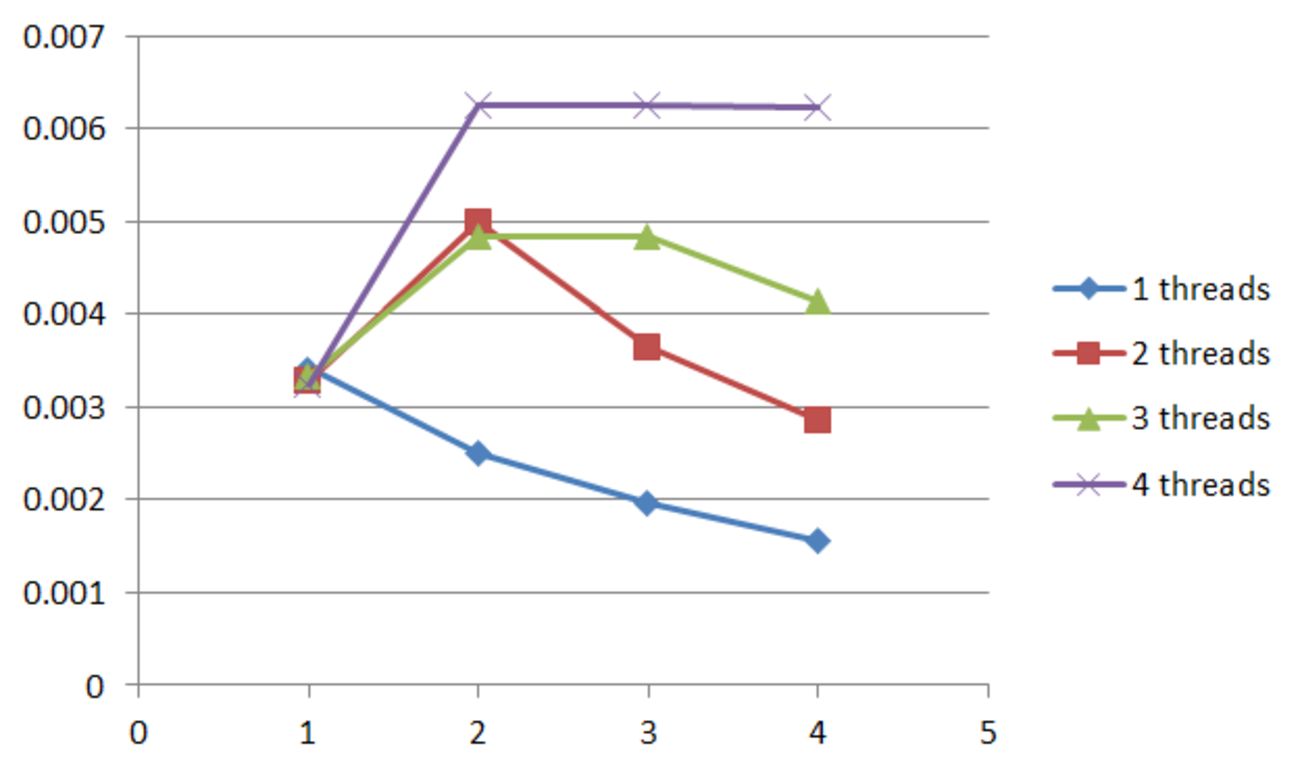
\includegraphics{figures/DynamicTaskPerCycle.pdf}}
\caption{{\bf Dynamic Interleave Task{\tt /}Cycle} The Y-Axis is in units of $task/cycle$.}
\label{fig:dynamicTaskPerCycle}
\centering
\resizebox{\columnwidth}{!}{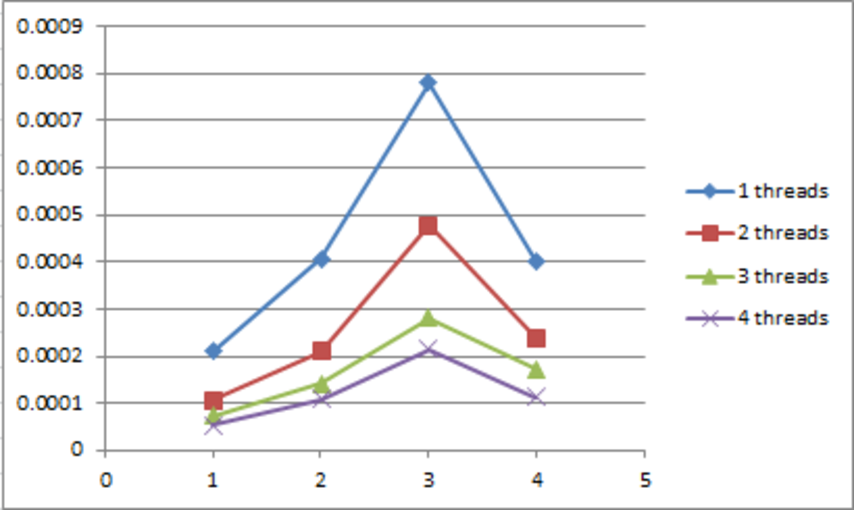
\includegraphics{figures/DynamicFreqPerArea.pdf}}
\caption{{\bf Dynamic Interleave (Cycle{\tt /}Time){\tt /}Area} The Y-Axis is in units of $GHz/um^2$.}
\label{fig:dynamicFreqPerArea}
\centering
\resizebox{\columnwidth}{!}{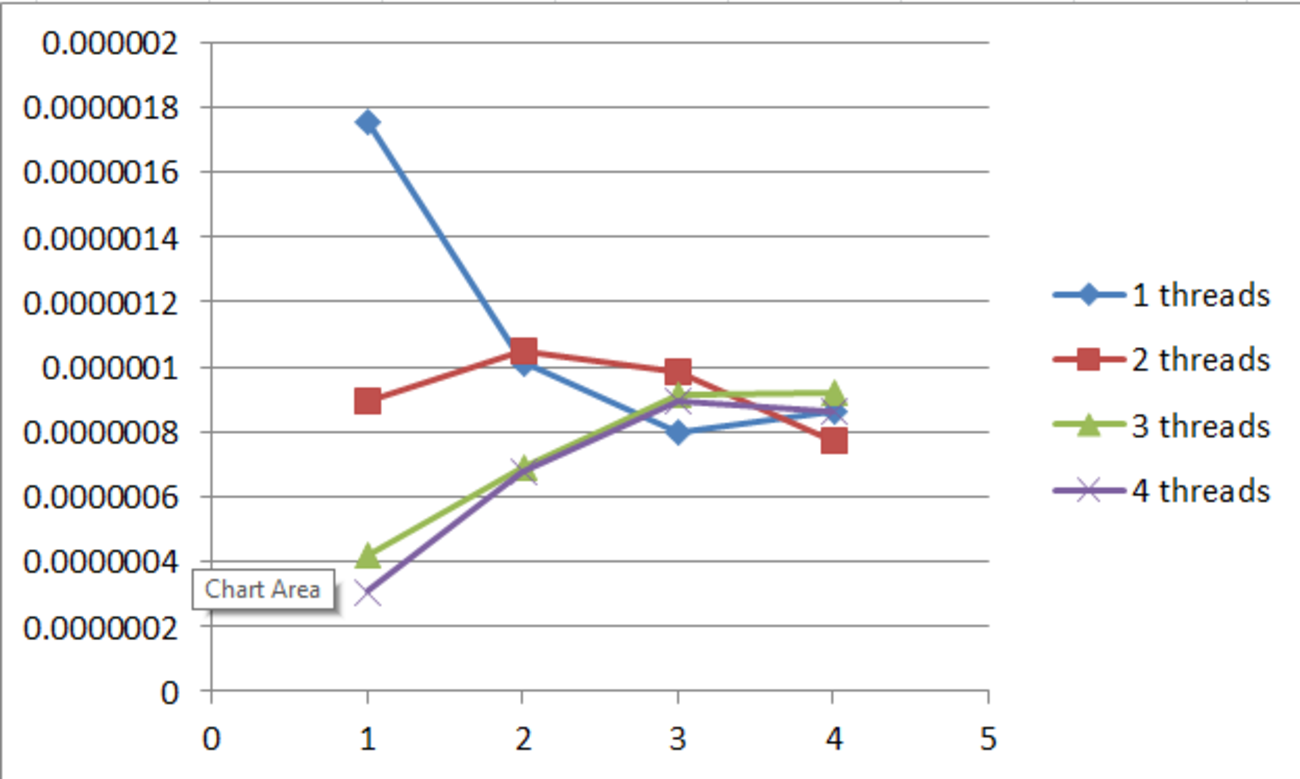
\includegraphics{figures/DynamicThroughputPerArea.pdf}}
\caption{{\bf Dynamic Interleave Throughput{\tt /}Area} The Y-Axis is in units of $(task/ns)/um^2$.}
\label{fig:dynamicThroughputPerArea}
\end{figure}

\begin{figure}
\centering
\resizebox{\columnwidth}{!}{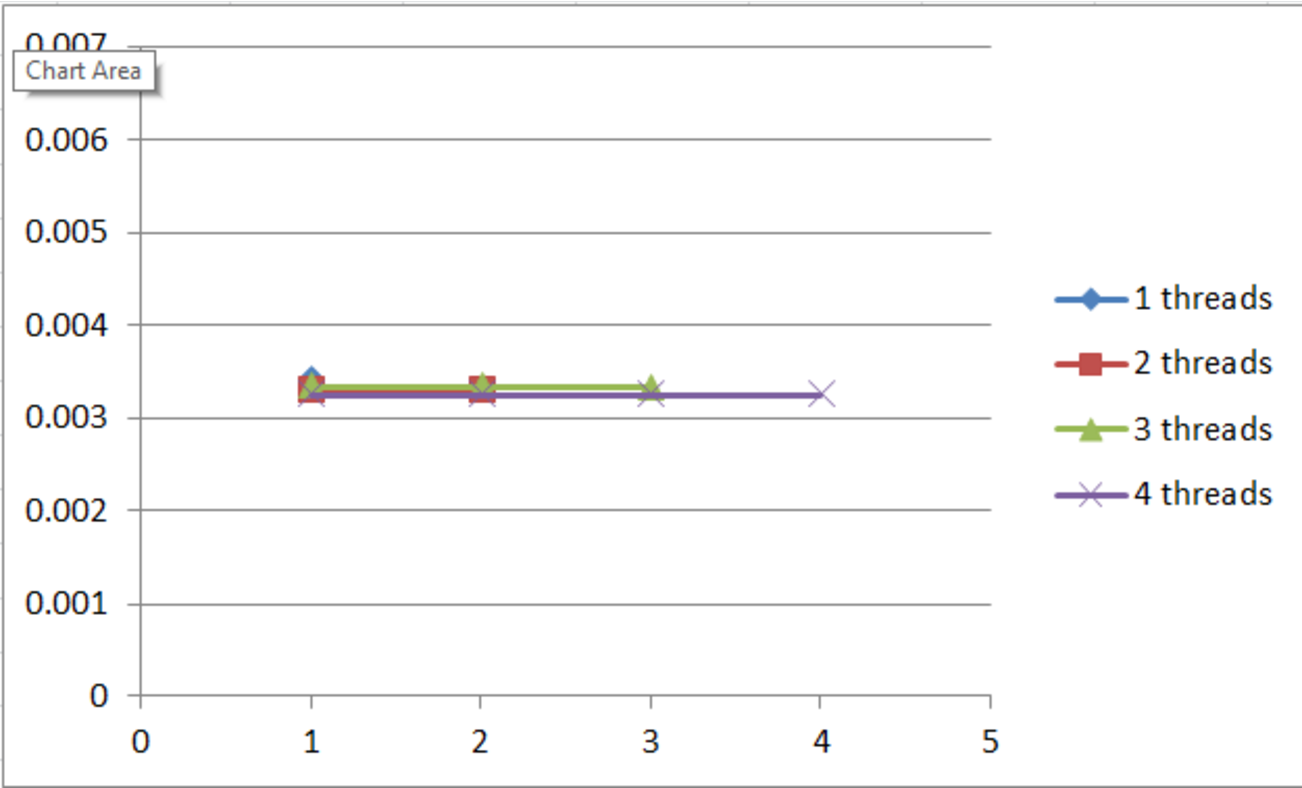
\includegraphics{figures/FixedTaskPerCycle.pdf}}
\caption{{\bf Fixed Interleave Task{\tt /}Cycle} The data points where number of stages {\tt >} number of threads are not valid design points for fixed interleave, so they do not exist on this chart. The Y-Axis is in units of $task/cycle$.}
\label{fig:fixedTaskPerCycle}
\centering
\resizebox{\columnwidth}{!}{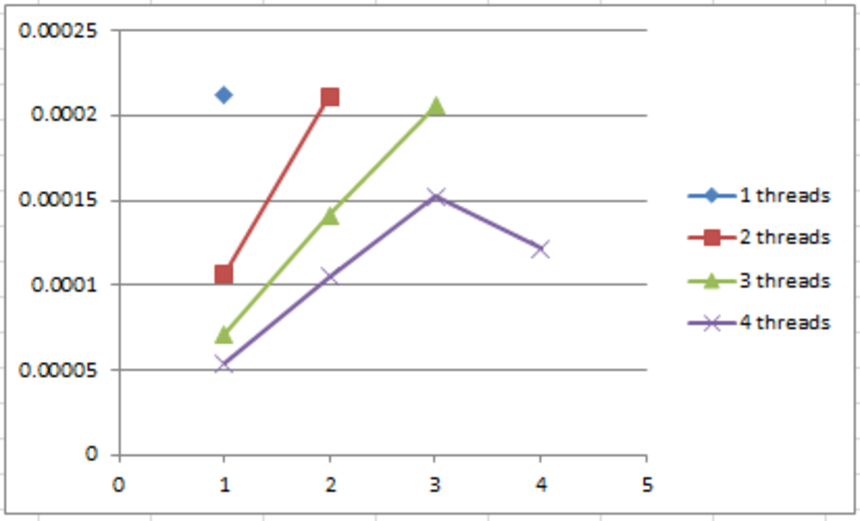
\includegraphics{figures/FixedFreqPerArea.pdf}}
\caption{{\bf Fixed Interleave (Cycle{\tt /}Time){\tt /}Area} The data points where number of stages {\tt >} number of threads are not valid design points for fixed interleave, so they do not exist on this chart. The Y-Axis is in units of $GHz/um^2$.}
\label{fig:fixedFreqPerArea}
\centering
\resizebox{\columnwidth}{!}{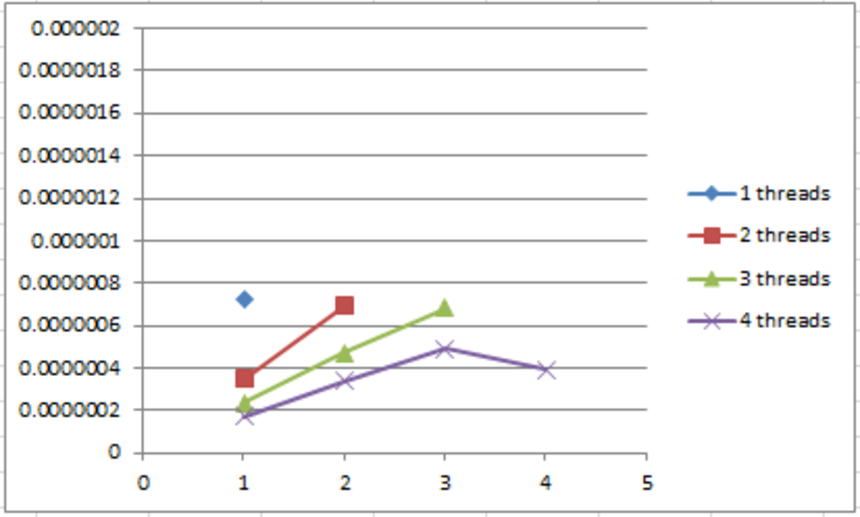
\includegraphics{figures/FixedThroughputPerArea.pdf}}
\caption{{\bf Fixed Interleave Throughput{\tt /}Area} The data points where number of stages {\tt >} number of threads are not valid design points for fixed interleave, so they do not exist on this chart. The Y-Axis is in units of $(task/ns)/um^2$.}
\label{fig:fixedThroughputPerArea}
\end{figure}




\section{Conclusion and Future Work}
In this thesis, I presented a system for digital circuit frontend specification named Automatic Functional Datapath Optimization. In this system, the designer specifies a base functionally correct datapath without any optimizations applied in a RTL like manner and then selects optimization techniques for automatic tools to apply to the base functional datapath. This system of specification is a middle ground approach between RTL specification and HLS specification and tries to capture the conflicting pros of both approaches, namely high designer productivity and the ability to generate highly efficient designs in terms of performance, power, and area at the same time. I implemented two examples of such a system, AutoMArch and AutoFAME, and presented example applications of both.

I hope that AutoMArch can be extended to support more general speculation and that a more general form multi-threading, where combinational logic is replicated as well as the state elements can be explored. I also hope that work can be done to catalogue all of the commonly used digital circuit optimization techniques so that they may one day be implemented automatically

\clearpage
\bibliographystyle{abbrvnat}
\setlength{\bibsep}{0.0pt}
\renewcommand*{\bibfont}{\footnotesize}
\bibliography{references}

\end{document}
